\customHeader{1}{\VSI{} Dataset}
\label{vsi_dataset}

As mentioned in \headerName{} \todo{Add reference here!}, the \gls{pesv} Platform collects information on any health risk or plant health phenomenon that could potentially affect agriculture. The epidemiologists achieve this by surveilling online articles, which they subsequently screen and collect into the \gls{vsi} dataset.

% %%%%%%%%%%%%%%%%%%%%%%%%%%%%%%%%%%%%%%%%%%%%%%%%%%%%%%%%%%%%%%%%%%%%%%%%%%%%%%%%%%%%%%
\customHeader{2}{Dataset Collection}
\label{vsi_data_collection}


The main tools for collecting documents are web scrapping and text mining. Every week, several queries are sent to the Google Search Engine, using the keywords and key phrases in Table \ref{tab:04_query_keywords}. 
The websites resulting from this Google Search are then manually analyzed by the epidemiologists and stored in the dataset. That is, the \gls{vsi} dataset is in constant construction. 
For this project, we worked with the documents collected from the 11th of July 2022 to the 16th of April 2023, that is, the data collected over 39 weeks.



\begin{table}%[]
    \centering
    %\begin{tabular}{|p|p|p|}
    \resizebox{\textwidth}{!}{
    \begin{tabular}{|p{0.3\textwidth}|c|p{0.4\textwidth}|}
    \hline
    \textbf{Organism of interest} &\textbf{Type of organism} & \textbf{Search Query} \\
    \hline
    
     Fusarium oxysporum f. sp. cubense tropical (race 4) &  Fungus &\cvtag{fusarium oxysporum tropical}  \\
     % https://en.wikipedia.org/wiki/Fusarium_oxysporum_f.sp._cubense#Tropical_Race_4/TR4
     Xylella fastidiosa & Bacteril & \cvtag{xylella}  \\
     % https://en.wikipedia.org/wiki/Xylella_fastidiosa
     Bursaphelenchus xylophilus &  Nematode & \cvtag{Bursaphelenchus xylophilus} \\
     % https://en.wikipedia.org/wiki/Bursaphelenchus_xylophilus
     Bactrocera dorsalis & Insect &  \cvtag{Bactrocera dorsalis} \\
     % https://en.wikipedia.org/wiki/Bactrocera_dorsalis
     Candidatus Liberibacter spp. &  Bacteria & \cvtag{huanglongbing} \\
     % https://en.wikipedia.org/wiki/Liberibacter
     Popillia japonica & Insect & \cvtag{Popillia Japonica} \\
     % https://en.wikipedia.org/wiki/Japanese_beetle
     Flavescence dor\'ee &  Bacteria  &  \cvtag{flavescence} \\
     % https://en.wikipedia.org/wiki/Flavescence_dor%C3%A9e
     Tomato brown rugose fruit virus &  Virus & \cvtag{ToBRFV}\\
     % https://en.wikipedia.org/wiki/Tomato_brown_rugose_fruit_virus
     Spodoptera frugiperda & Insect & \cvtag{spodoptera frugiperda} \\
     % https://en.wikipedia.org/wiki/Fall_armyworm
     Bretziella fagacearum & Fungus & \cvtag{oak wilt Bretziella} \\
     % https://wiki.pestinfo.org/wiki/Bretziella_fagacearum
     Agrilus planipennis & Insect & \cvtag{Agrilus planipennis}  \\
     % https://en.wikipedia.org/wiki/Emerald_ash_borer
     Thaumatotibia leucotreta & Insect &  \cvtag{Thaumatotibia leucotreta} \\
     % https://en.wikipedia.org/wiki/False_codling_moth
     Xylotrechus chinensis & Insect & \cvtag{Xylotrechus chinensis}  \\
     % https://es.wikipedia.org/wiki/Xylotrechus_chinensis
     Toumeyella parvicornis & Insect & \cvtag{Toumeyella parvicornis}  \\
     % https://en.wikipedia.org/wiki/Toumeyella_parvicornis
     Ceratocystis platani & Fungus &  \cvtag{Ceratocystis platani}  \cvtag{chancre du platane}  \\ \hline
     % https://en.wikipedia.org/wiki/Ceratocystis_platani
     General Plant Health & \  &\cvtag{first report plant disease} \cvtag{new plant health}   \\
    \hline
    \end{tabular}
    }
    \caption{Keywords and key phrases used for the \VSI dataset}
    \label{tab:04_query_keywords}
\end{table}



The query results are then scrapped using the tool \trafilatura{} \myparencite{barbaresi-2021-trafilatura}, which attempts to extract a title, an abstract, the full text, and other data from the websites.
Specifically, for a website, \trafilatura{} scrapes the HTML content and parses it into XML. The tool then extracts the title and abstract from the XML metadata\footnote{The title and the abstract are extracted from the \texttt{metadata.title} and \texttt{metadata.description} fields, respectively.} and the full text from the XML body.
Given that these articles come from public websites, all the content is in its original language.
In order to help the annotators make a decision when encountering an article in a foreign language, and due to budget limitations, only the title is translated to English, using the Google Translate API. Thus, we have four sources of text content (Table \ref{tab:04_pesv_sources of content}).

\begin{table}%[]
    \centering
    \begin{tabular}{c|c}
       \textbf{\contentType{}}  & \textbf{Tool} \\ \hline
       \trafilaturaTitle{}  & Trafilatura \\
       \trafilaturaAbstract{}  & Trafilatura \\
       \trafilaturaFulltext{}  & Trafilatura \\
       \translationTitle{}  & Google Translate \\
    \end{tabular}
    \caption{Sources of text content in the \VSI{} Dataset}
    \label{tab:04_pesv_sources of content}
\end{table}




% %%%%%%%%%%%%%%%%%%%%%%%%%%%%%%%%%%%%%%%%%%%%%%%%%%%%%%%%%%%%%%%%%%%%%%%%%%%%%%%%%%%%%%
\customHeader{2}{Dataset Annotation}
\label{vsi_data_annotation}

There are four epidemiologists dedicated to annotating the dataset: 

\begin{itemize}
    \item \todo{add names of epidemiologists}
    \item \todo{add names of epidemiologists}
    \item \todo{add names of epidemiologists}
    \item \todo{add names of epidemiologists}
\end{itemize}


After obtaining results from the Google Search, the epidemiologists are presented with the URL of an article, which they manually open and proceed to read. Using the interface in Figure \ref{fig:04_pesv_interface_1}, they fill out the fields \emph{Titre} (title), \emph{Auteurs} (authors), \emph{Organism nuisible} (pathogen), \emph{Sujet} (subject), \emph{Fiabilité} (trustworthyness), etc. 
It is important to note that the title written by the epidemiologists is usually different from the one extracted by \trafilatura{} (for example, they may include different characters). Other fields, like \emph{Date de publication} (publication date) and \emph{Lien} (link) are filled automatically.

After inspection, we found that that annotators exclusively provide titles for articles they find relevant, that is, there are no titles for irrelevant articles. Since our objective is to automate the process of identifying relevant articles, we disregard the titles provided by the annotators. Instead, we rely solely on the titles generated by \trafilatura{} and Google Translate, which are stored even in the case of the documents being rejected.

Special attention must be given to the \emph{Sujet} (subject), as this field will be crucial for preprocessing the dataset (see \headerName{} \ref{vsi_resolving_inconsistencies}).

\begin{tcolorbox}[colback=mylightblue,colframe=gray!50!black]
As part of their monitoring mission \todo{add reference to the Introduction}, the \gls{pesv} Platform surveys any health risk or plant health phenomenon that has or may have an impact on agriculture. 
When the epidemiologists encounter an event that catches their attention (that is, that they consider \textbf{relevant}), they assign a \textbf{subject} to the respective document and utilize the interface presented in Figure \ref{fig:04_pesv_interface_2} to allocate a subject ID and description to it. It is possible for multiple documents to share the same subject. In the case of documents considered \textbf{irrelevant} to the monitoring of plant health, the subject field for the document is left empty.
\end{tcolorbox}
Some sample entries containing all sources of content can be found in Table \ref{tab:04_sample_entries_vsi}.

\begin{landscape}
    \begin{figure}[ht]
        \centering
        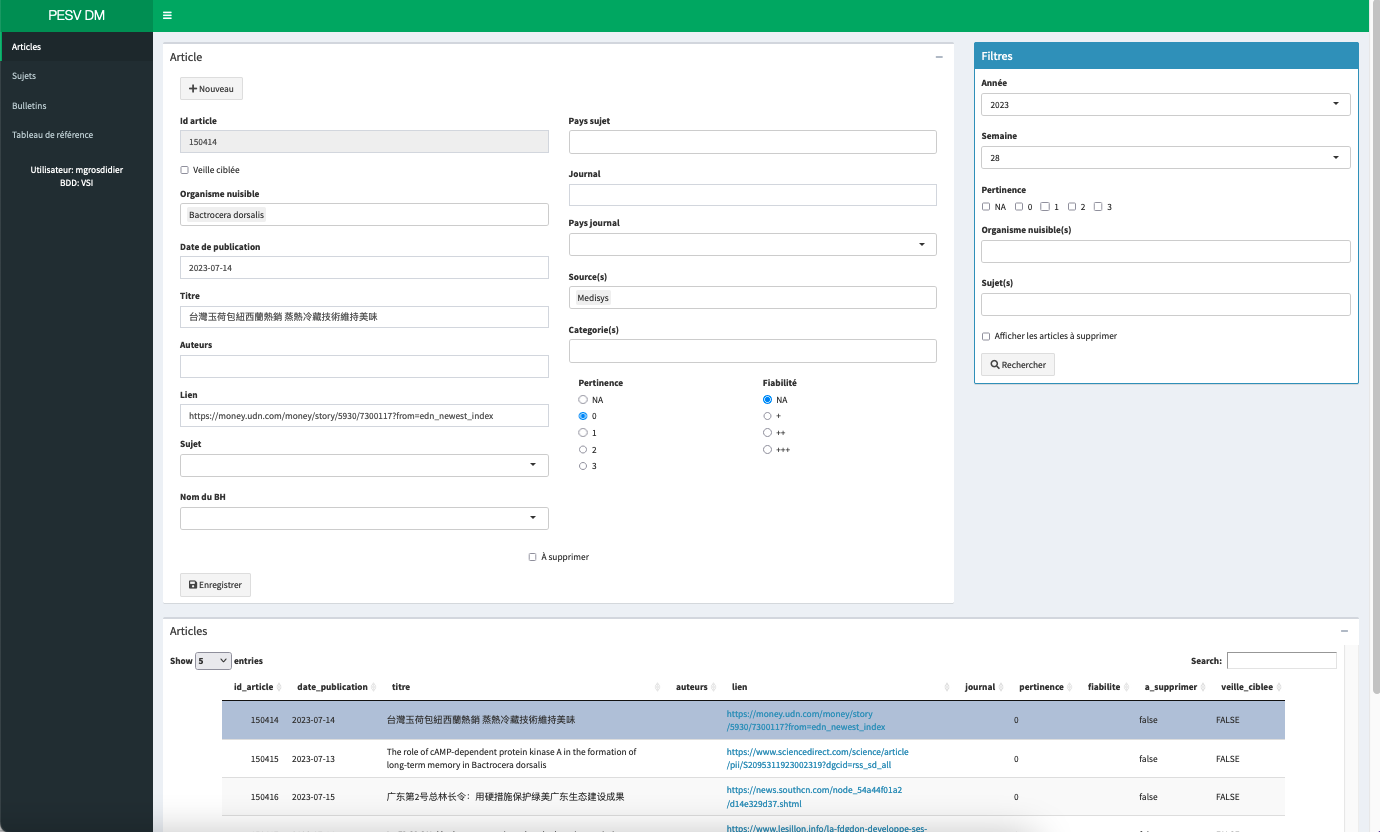
\includegraphics[width=1.20\textwidth]{Figures/04/PESV_interface_1.png}
        \caption{\VSI{} Annotation Interface for Articles}
        \label{fig:04_pesv_interface_1}
    \end{figure}
\end{landscape}

\begin{landscape}
    \begin{figure}[ht]
        \centering
        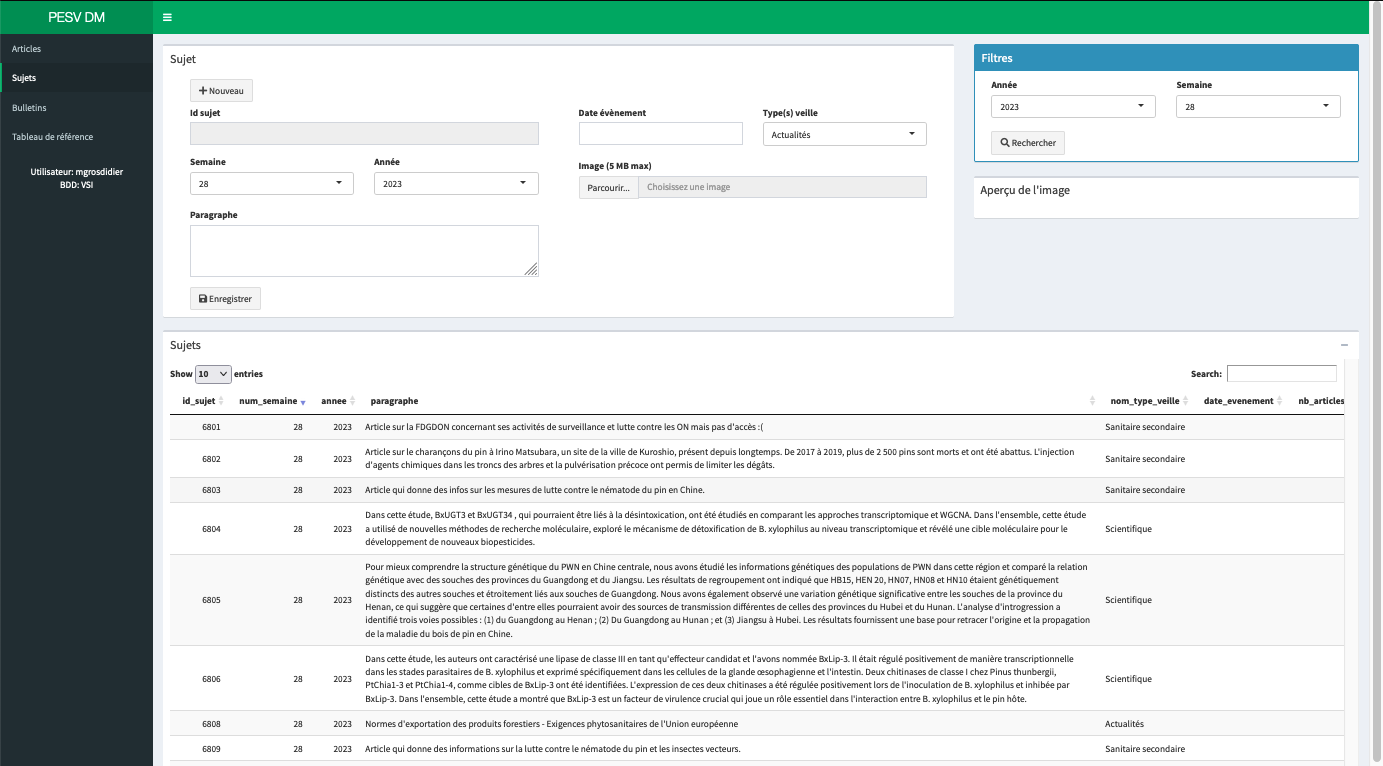
\includegraphics[width=1.20\textwidth]{Figures/04/PESV_interface_2.png}
        \caption{\VSI{} Annotation Interface for Subjects}
        \label{fig:04_pesv_interface_2}
    \end{figure}
\end{landscape}


\begin{landscape}
\begin{table}%[]
\resizebox{\paperwidth}{!}{

\begin{tabular}{|c|p{4cm}|p{4cm}|p{5cm}|p{5cm}|c|}
\hline
\textbf{Entry ID} & \textbf{\trafilaturaTitle{}} & \textbf{\translationTitle{}} & \textbf{\trafilaturaAbstract{}} & \textbf{\trafilaturaFulltext{}} & \textbf{Subject ID} \\
\hline
68 & Xylella, da giugno 47 nuovi casi & Xylella, 47 new cases since June & In Puglia la Xylella fa\ldots & Xylella, da giugno 47 nuovi casiIn Puglia\ldots & 4279 \\ \hline
305 & Agro - EL HERALDO - Edizione digitale & Agro - EL HERALDO - Digital edition & EL HERALDO - Edizione digital\ldots & El presidente de la Federación del Citrus\ldots & None \\ \hline
320 & Misure fitosanitarie di controllo della Popillia japonica - 2022 & Phytosanitary measures to control Popillia japonica - 2022 & Il Servizio Fitosanitario Regionale per\ldots & Popillia japonica è un insetto originario del\ldots & 4286 \\ \hline
177 & Traps set to catch invasive, destructive fruit fly in Pinellas County & Traps set to catch invasive, destructive fruit fly in Pinellas County & Florida Agriculture leaders are on\ldots & PINELLAS COUNTY, Fla. — Florida Agriculture leaders\ldots & None \\ \hline
159 & Preocupan los efectos del cambio climático en la variedad picual & The effects of climate change on the picual variety are of concern & Podría ver reducido su rendimiento\ldots & 1. ¿Qué son las cookies? La Web\ldots & None \\ \hline
89 & Frantoi di Puglia danneggiati dalla Xylella, in arrivo 35 milioni di euro & Puglia oil mills damaged by Xylella, 35 million euros on the way & I frantoi oleari della Puglia\ldots & I frantoi oleari della Puglia potranno presto\ldots & None \\ \hline
82 & Dal Mipaaf un miliardo per i terreni colpiti da Xylella & From Mipaaf one billion for the land affected by Xylella & Dal Mipaaf un miliardo per\ldots & Il V bando per i Contratti di\ldots & None \\ \hline
61 & Le ministère veut alerter sur les espèces invasives & The ministry wants to warn about invasive species & Le ministère de l’Agriculture lance\ldots & « Plantes en danger » Le ministère\ldots & None \\ \hline
78 & Xylella, casi di Polignano portano più a nord il limite della Puglia & Xylella, cases of Polignano bring the limit of Puglia further north & Il piano di Emergenza evidenzia\ldots & In Puglia e Basilicata SOS AGRICOLTURA Resta\ldots & 4279 \\
\hline
\end{tabular}
}
    \caption{Sample entries from the \VSI{} dataset}
    \label{tab:04_sample_entries_vsi}
\end{table}
\end{landscape}


% %%%%%%%%%%%%%%%%%%%%%%%%%%%%%%%%%%%%%%%%%%%%%%%%%%%%%%%%%%%%%%%%%%%%%%%%%%%%%%%%%%%%%%
\customHeader{2}{Dataset Stastitics}
\label{vsi_data_statistics}

There are 34587 entries in the dataset, out of which 3715 have an assigned subject and 30872 do not, producing a highly unbalanced dataset (Figure \ref{fig:04_naive_positives_and_negatives}). 

\begin{figure}
    \centering
    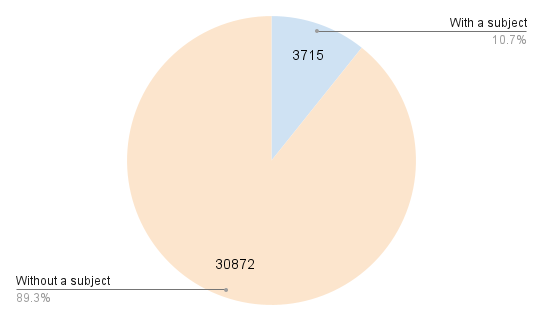
\includegraphics[width=0.75\textwidth]{Figures/04/naive_positives_and_negatives_chart.png}
    \caption{Distribution of subjects in the \VSI{} dataset without preprocessing}
    \label{fig:04_naive_positives_and_negatives}
\end{figure}

The automatic language detection obtained by the Google Translate API  on the \trafilaturaTitle{} can be used to approximately study the distribution of the entries in the dataset. In Figure \ref{fig:04_vsi_language_distribution} it can be seen that around one third of the entries are in English, followed by Italian, Spanish, and French. There is a considerable amount of failed translation attempts, for around one fifth of the entries. The complete data on documents per language is available in Appendix \ref{appendix01:vsi_language_distribution}.
 
\begin{figure}
    \centering
    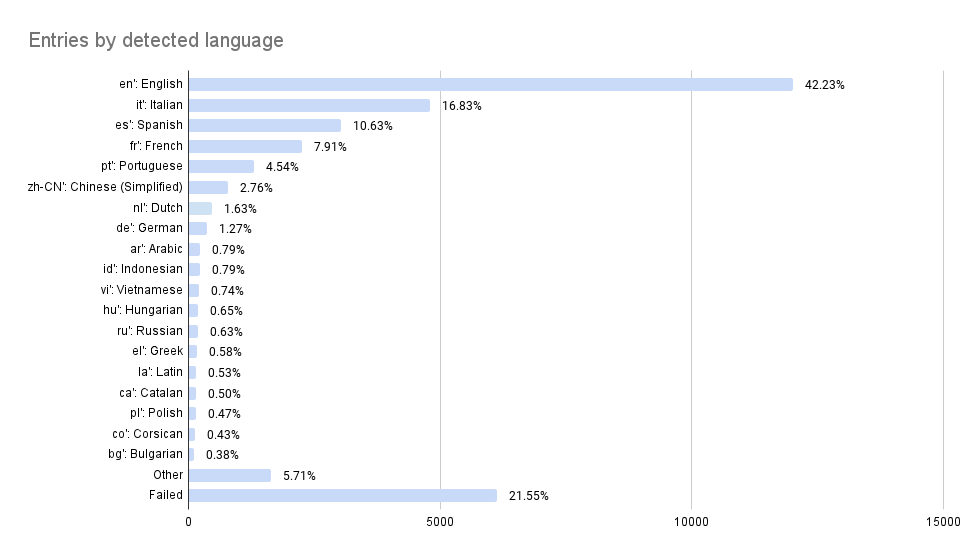
\includegraphics[width=0.75\textwidth]{Figures/04/Entries by detected language.png}
    \caption{Language distribution of entries in the \VSI{} dataset}
    \label{fig:04_vsi_language_distribution}
\end{figure}

The presence of some Latin documents is surprising. Upon inspecting the data, we discovered that this occurrence was due to scrapped \trafilaturaTitle{}s with several scientific names (Table \ref{tab:appendix01:latin_entries} in the Appendix).

Often, the \trafilatura{} scrapper is not able to retrieve content for the title, abstract, and full text of a website, or the Google Translate API fails. Thus, there are several entries without content for all fields. If we check the unique entries for each source of content, we can see that there must be numerous duplicate entries, since there are at least around 20 000 unique entries per source of content (Figure \ref{fig:04_unique_entries_vsi}).

\begin{figure}
    \centering
    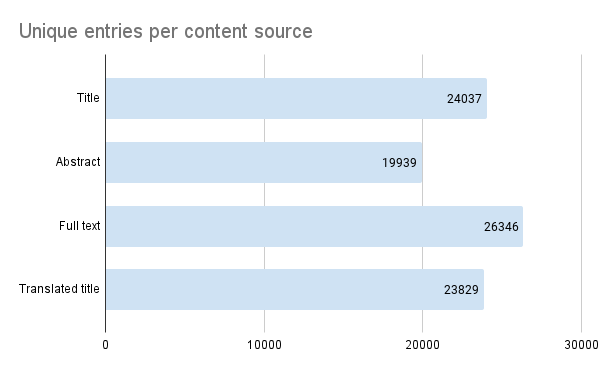
\includegraphics[width=0.50\textwidth]{Figures/04/Unique entries per content source.png}
    \caption{Unique entries per source of content in the \VSI{} dataset}
    \label{fig:04_unique_entries_vsi}
\end{figure}

As one would expect, there are fewer unique entries for the \translationTitle{} as there are for the \trafilaturaTitle{}. At the same time, the \trafilaturaAbstract{} field has fewer unique entries than all the other, while the \trafilaturaFulltext{} has the most. This may be explained by the fact that, usually, the creators of a website omit filling the metadata, and when they do, they frequently include only a title and not a description, while most times, the body of the website will be available. 

Using naive tokenization (splitting on whitespace), we can study the distribution of the tokens for all sources of content. In the histograms in Figure \ref{fig:04_vsi_token_distribution} the longest documents have been grouped together to facilitate plotting \footnote{This explains the long bars at the end of the right tails of the histograms.}. As one can see, the \trafilaturaTitle{} and \translationTitle{} have a very similar distribution, both are shorter than the \trafilaturaAbstract{}, while the content from the \trafilaturaFulltext{} is the longest.

\begin{figure}[ht]
    \centering
    \subfigure[\trafilaturaTitle{}]{
        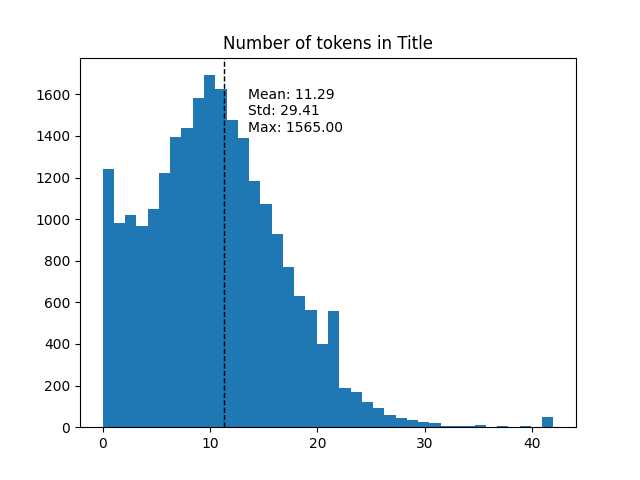
\includegraphics[width=0.45\textwidth]{Figures/04/Histograms/length histogram parsed_trafilatura_title.png}
        %\label{fig:image1}
    }
    \hfill
    \subfigure[\trafilaturaAbstract{}]{
        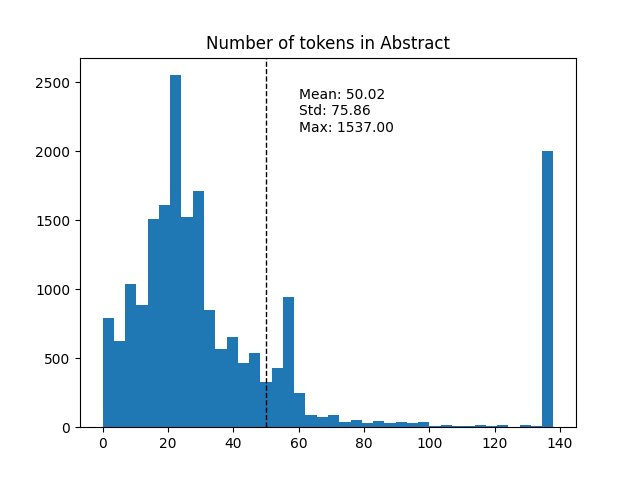
\includegraphics[width=0.45\textwidth]{Figures/04/Histograms/length histogram parsed_trafilatura_abstract.png}
        %\label{fig:image2}
    }
    
    \subfigure[\trafilaturaFulltext{}]{
        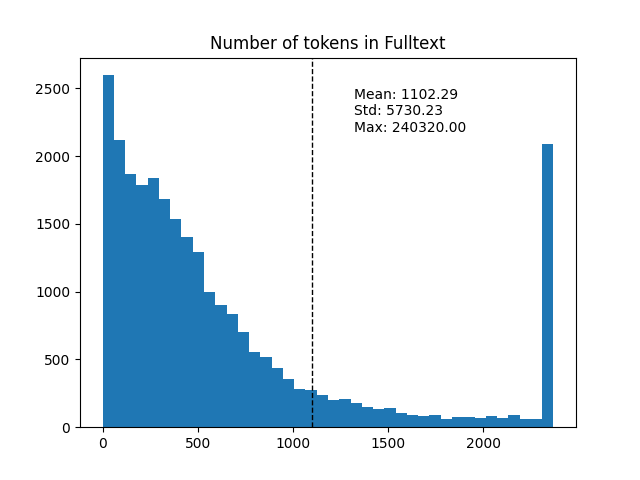
\includegraphics[width=0.45\textwidth]{Figures/04/Histograms/length histogram parsed_trafilatura_fulltext.png}
        %\label{fig:image3}
    }
    \hfill
    \subfigure[\translationTitle{}]{
        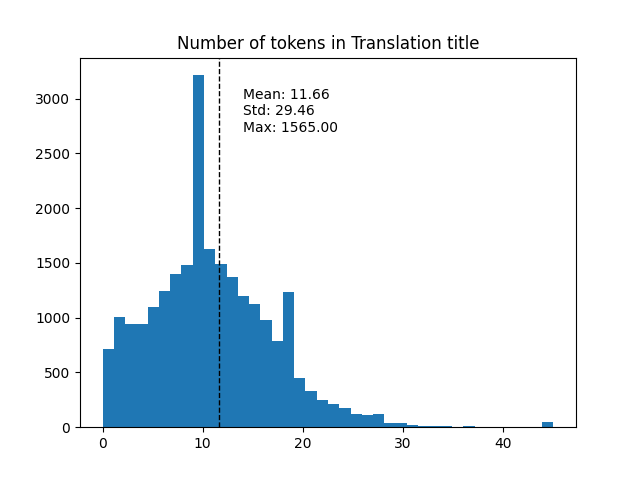
\includegraphics[width=0.45\textwidth]{Figures/04/Histograms/length histogram translation_title.png}
        %\label{fig:image4}
    }
    
    \caption{Token distribution in the \VSI{} dataset}
    \label{fig:04_vsi_token_distribution}
\end{figure}





\begin{tcolorbox}[colback=mylightblue,colframe=gray!50!black]
Regrettably, while constructing the dataset, there was no record maintained to track the identity of the annotator responsible for labelling each document. For this reason, we are not able to provide any inter-annotator agreement measures on this dataset \myparencite{agreement_measures}.
\end{tcolorbox}

% %%%%%%%%%%%%%%%%%%%%%%%%%%%%%%%%%%%%%%%%%%%%%%%%%%%%%%%%%%%%%%%%%%%%%%%%%%%%%%%%%%%%%%
\customHeader{2}{Dataset Issues}
\label{vsi_data_issues}


Upon examining the data, we encountered numerous issues that we proceed to describe and which will be addressed during preprocessing in \headerName{} \ref{vsi_preprocessing}.


\customHeader{3}{Duplicate Entries}
\label{vsi_issues_duplicates}
\ \\

As mentioned in \headerName{} \ref{vsi_data_statistics}, there are numerous duplicate entries in the dataset (Figure \ref{fig:04_naive_positives_and_negatives} VS Figure \ref{fig:04_unique_entries_vsi}). According to the epidemiologists, often the Google Search for a query will return the same results from one week to the next, and this introduces duplicate entries.
 


\customHeader{3}{Scrapping Failures}
\label{vsi_issues_error_messages}
\ \\

On numerous instances, the \trafilatura{} scrapper either fails or is blocked by website servers that do not allow bots. This introduces error messages to the dataset, some samples of which can be seen in Table \ref{tab:04_error_messages}.

\begin{table}[ht]
\centering
\begin{tabular}{|c|}

\hline
\textbf{Error Message}\\ \hline
Not Found \\
404 \\
Page Not Found \\
Your data. Your experience. \\
Loading... \\
None \\
nan \\
JavaScript n'est pas disponible. \\
JavaScript is not available. \\
Please update your browser \\
Do you accept cookies ?\\
Verify you are not a robot\\
Discuz! Database Error\\
\hline
\end{tabular}
\caption{Some error messages in the \VSI{} dataset}
\label{tab:04_error_messages}
\end{table}



\customHeader{3}{Scrapping errors}
\label{vsi_issues_scrapping_errors}
\ \\

In some other instances, the web scraper successfully extracts content from the website, but the parsing algorithm performs poorly, retrieving only the headers or the website's name (Tables \ref{tab:04_headers} and \ref{tab:04_website_names}).


\begin{table}[ht]
\centering
\begin{minipage}{0.45\linewidth}
\centering
\begin{tabular}{|c|}
\hline
\textbf{Header} \\ \hline
Search results \\
Welcome \\
Advance articles \\
shop \\
Green Blog \\
Pesquisa (\textit{Query})\\
Link Diretti (\textit{Direct Links})\\
Búsqueda (\textit{Query})\\
Actualidad (\textit{Current events})\\
Browsing \\
Project Listing \\
Research articles \\
Pagamenti Online (\textit{Online Payments})\\
Notícias (\textit{News})\\
Category: events \\
News \\
\hline
\end{tabular}
\caption{Some headers parsed by \trafilatura{} }
\label{tab:04_headers}
\end{minipage}
\hfill
\begin{minipage}{0.45\linewidth}
\centering
\begin{tabular}{|c|}
\hline
\textbf{Website name} \\ \hline
Wall Street Journal \\
Bloomberg \\
TikTok \\
Facebook \\
Portal Embrapa \\
Argentina.gob.ar \\
Notizie dal Comune (\textit{Town News}) \\
zmianynaziemi.pl \\
Pakistan Journal of Zoology \\
SAARC Journal of Agriculture \\
MONTSAME News Agency \\
ORCID \\
\hline
\end{tabular}
\caption{Some website names parsed by \trafilatura{} }
\label{tab:04_website_names}
\end{minipage}
\end{table}



This introduces inconsistencies into the \VSI{} dataset. In cases where multiple documents originate from the same problematic website, the original content is lost, and we encounter entries that contain identical text but carry different assigned subjects, as in Table \ref{tab:04_xmol_inconsistencies}\footnote{\href{https://www.x-mol.com/}{X-MOL} is a Chinese search engine for scholars.}.




\begin{landscape}
\begin{table}%[]
\resizebox{\paperwidth}{!}{
\begin{tabular}{llp{2cm}lll}
 \textbf{Entry ID}     & \textbf{\trafilaturaTitle{}} & \textbf{\translationTitle{}} & \textbf{\trafilaturaAbstract{}}  & \textbf{\trafilaturaFulltext{}}                      & \textbf{Subject}  \\ \hline
12895 & X-MOL              & X-MOL                & Web site created using create-react-app & X-MOLYou need to enable JavaScript to run this app. &  None      \\
13860 & X-MOL              & X-MOL                & Web site created using create-react-app & X-MOLYou need to enable JavaScript to run this app. & 4827 \\
14614 & X-MOL              & X-MOL                & Web site created using create-react-app & X-MOLYou need to enable JavaScript to run this app. & 4874 \\
15033 & X-MOL              & X-MOL                & Web site created using create-react-app & X-MOLYou need to enable JavaScript to run this app. & 4896 \\
15271 & X-MOL              & X-MOL                & Web site created using create-react-app & X-MOLYou need to enable JavaScript to run this app. & None       \\
15683 & X-MOL              & X-MOL                & Web site created using create-react-app & X-MOLYou need to enable JavaScript to run this app. & 4930 \\
16355 & X-MOL              & X-MOL                & Web site created using create-react-app & X-MOLYou need to enable JavaScript to run this app. & 4984 \\
16472 & X-MOL              & X-MOL                & Web site created using create-react-app & X-MOLYou need to enable JavaScript to run this app. & None       \\
19065 & X-MOL              & X-MOL                & Web site created using create-react-app & X-MOLYou need to enable JavaScript to run this app. & None       \\
19541 & X-MOL              & X-MOL                & Web site created using create-react-app & X-MOLYou need to enable JavaScript to run this app. & None       \\
21913 & X-MOL              & X-MOL                & Web site created using create-react-app & X-MOLYou need to enable JavaScript to run this app. & 5186 \\
22152 & X-MOL              & X-MOL                & Web site created using create-react-app & X-MOLYou need to enable JavaScript to run this app. & None       \\
23491 & X-MOL              & X-MOL                & Web site created using create-react-app & X-MOLYou need to enable JavaScript to run this app. & None       \\
23745 & X-MOL              & X-MOL                & Web site created using create-react-app & X-MOLYou need to enable JavaScript to run this app. & None       \\
25632 & X-MOL              & X-MOL                & Web site created using create-react-app & X-MOLYou need to enable JavaScript to run this app. & None       \\
26284 & X-MOL              & X-MOL                & Web site created using create-react-app & X-MOLYou need to enable JavaScript to run this app. & 5448 \\
29990 & X-MOL              & X-MOL                & Web site created using create-react-app & X-MOLYou need to enable JavaScript to run this app. & 5694 \\
30419 & X-MOL              & X-MOL                & Web site created using create-react-app & X-MOLYou need to enable JavaScript to run this app. & 5686 \\
30456 & X-MOL              & X-MOL                & Web site created using create-react-app & X-MOLYou need to enable JavaScript to run this app. & None       \\
30994 & X-MOL              & X-MOL                & Web site created using create-react-app & X-MOLYou need to enable JavaScript to run this app. & 5743 \\
31122 & X-MOL              & X-MOL                & Web site created using create-react-app & X-MOLYou need to enable JavaScript to run this app. & None       \\
31543 & X-MOL              & X-MOL                & Web site created using create-react-app & X-MOLYou need to enable JavaScript to run this app. & None       \\
32019 & X-MOL              & X-MOL                & Web site created using create-react-app & X-MOLYou need to enable JavaScript to run this app. & 5757 \\
32096 & X-MOL              & X-MOL                & Web site created using create-react-app & X-MOLYou need to enable JavaScript to run this app. & 5799 \\
32279 & X-MOL              & X-MOL                & Web site created using create-react-app & X-MOLYou need to enable JavaScript to run this app. & None       \\
32495 & X-MOL              & X-MOL                & Web site created using create-react-app & X-MOLYou need to enable JavaScript to run this app. & None       \\
33089 & X-MOL              & X-MOL                & Web site created using create-react-app & X-MOLYou need to enable JavaScript to run this app. & 5829 \\
34431 & X-MOL              & X-MOL                & Web site created using create-react-app & X-MOLYou need to enable JavaScript to run this app. & None      
\end{tabular}
}
\caption{Inconsistencies introduced by scrapping errors}
\label{tab:04_xmol_inconsistencies}
\end{table}
\end{landscape}




\customHeader{3}{Data Noise}
\label{vsi_issues_data_noise}
\ \\

Even in those cases when \trafilatura{} is able to retrieve content from the website, there are some expected types of noise in the data, considering it comes from the internet.
Namely, the following  (Table \ref{tab:04_noise}) :
\begin{itemize}
    \item URLs
    \item HTML Tags
    \item Emojis
    \item Encoding errors
    \item Generic noise (different quotation or division characters, strings containing only dates, etc\ldots)
\end{itemize}




% endings - pubmed
% URLs, tags, emojis



\begin{table}[!htbp]
\centering
\begin{tabular}{|p{\textwidth}|}
\hline
\multicolumn{1}{|c|}{URLs} \\
\hline
'Regione attiva piano anti Popillia japonica - www.lombardianotizie.online - Conflombardia\\
'SciELO Argentina - www.scielo.org.ar\\
'https://twitter.com/julia\_lopez9/status/1601582135923863553/photo/1\\
%'Иновативен пъпеш на пазара - www.economynews.bg\\
'Ornitho.it homepage - www.ornitho.it\\
'Dzienna porcja warzyw - Nasza Rola - www.naszarola.pl\\
\hline
\end{tabular}

\vspace{0.5cm}

\begin{tabular}{|p{\textwidth}|}
\hline
\multicolumn{1}{|c|}{HTML Tags} \\
\hline
$<$strong$>$Fall armyworm in Europe: how can we use biocontrol? $<$/strong$>$\\
$<$strong$>$Xylella, CIA Puglia: $<$/strong$>$«$<$strong$>$Presidente Emiliano se ci sei batti un colpo$<$/strong$>$»\\
Japankäfer $<$i$>$Popillia japonica$<$/i$>$\\
Categoría: $<$span$>$Revista$<$/span$>$\\
Corteva Agriscience introduces seed treatment product Dermacor$<$sup$>$®$<$/sup$>$ in Brazil\\
Current Research on $<$em$>$Fusarium$<$/em$>$\\
{[Other]} Highly Sensitive and Rapid Detection of Citrus Huanglongbing Pathogen ($<$i$>$Candidatus$<$/i$>$ Liberibacter asiaticus’) Using Cas12a-Based Methods\\
\hline
\end{tabular}

\vspace{0.5cm}

\begin{tabular}{|p{\textwidth}|}
\hline
\multicolumn{1}{|c|}{Emojis} \\
\hline
Esther Ogunbayo on LinkedIn: https://lnkd.in/dEwvQD\_A Adeoye Opeyemi kindly like, follow and repost 
\emoji{grinning-face} \\
{[ \emoji{star} ]} on TikTok \\
``\#Leonardo \#italy\emoji{flag-italy} \#puglia \#taranto \#volgopuglia \#volgoitalia | Lion sculpture, Sculpture, Taranto"\\
\emoji{scientist}\emoji{microscope}\emoji{test-tube}Gen L de resistencia al Virus Rugoso del Tomate (ToBRFV)\emoji{microbe} | Agrocultivos TV innovando\\
\hline
\end{tabular}

\vspace{0.5cm}

\begin{tabular}{|p{\textwidth}|}
\hline
\multicolumn{1}{|c|}{Encoding Errors} \\
\hline
$<$º°Ç¥ 3$>$ ¹®Àå(Á¦6Á¶°ü·Ã).\\
Pomidorų vaisiaus rudųjų raukÅ¡lių virusas â vienas pavojingiausių\\
âç½çº¢âé³éé³éâå ¨å½å´æâ é²æ²»ä¸è½âä¸æäºäºâ\\
æµè¥¿ä¹¡ææºåå¤æ ç®¡æ¤ è¶ åç¾æ£µç¾å¹´å¤æ âèææä¾â\\
ç山人é¿åºâç§æ翼â æ¹åå²³é³å¿â红è¢ç« âå®æ¤â森æ绿â\\
Το ÎÎΩΤÎÎ ÎÏήÏÎ·Ï Î´Î¯Î½ÎµÎ¹ ÏÏÏÏÎ¿Ï Ï Î±Î½ÏιμεÏÏÏιÏÎ·Ï ÏÎ¿Ï Î´Î¬ÎºÎ¿Ï ÏÎ·Ï ÎµÎ»Î¹Î¬Ï - §Î±Î½Î¹ÏÏικα ÎÎα\\
客æ·å表æç®\\
\hline
\end{tabular}
\caption{Noise in the \VSI{} dataset}
\label{tab:04_noise}
\end{table}


However, an unforeseen form of noise arises: occasionally, the content concludes with the website's name, leading to different entries that vary by only a few tokens as a suffix (Table \ref{tab:04_website_names_as_suffixes}).

\begin{table}[!htbp]
  \centering
  \begin{tabular}{p{\textwidth}}
    \hline
    \textbf{\trafilaturaTitle{}} \\
    \hline
    Cousin of crop-killing bacteria mutating rapidly \\
    Cousin of crop-killing bacteria mutating rapidly - MixPoint \\
    Cousin of crop-killing bacteria mutating rapidly - My Droll \\
    Cousin of crop-killing bacteria mutating rapidly - Newsprepare \\
    Cousin of crop-killing bacteria mutating rapidly - Sky News: The Latest News from the World \\
    Cousin of crop-killing bacteria mutating rapidly - timetotimes.com \\
    \hline
    Modeling climate change impacts on potential global distribution of Tamarixia radiata \\
    Modeling climate change impacts on potential global distribution of Tamarixia radiata - PubMed \\
    \hline
    Portugal detecta Xylella en cítricos por primera vez en la UE y en Italia se consolida el foco de ‘Mosca oriental’\\
    Portugal detecta Xylella en cítricos por primera vez en la UE y en Italia se consolida el foco de ‘Mosca oriental’ - Agrodigital \\
    \hline
    Portugal detecta Xylella en 75 especies vegetales\\
    Portugal detecta Xylella en 75 especies vegetales - FruitToday \\
    \hline
    Tornano le Giornate Fai di Primavera: 750 luoghi aperti in tutta Italia\\
    Tornano le Giornate Fai di Primavera: 750 luoghi aperti in tutta Italia - LegnanoNews \\
    \hline
    Giornate Fai di Primavera. I segreti dell'edizione 2023. Da Bolzano alla Sardegna, 750 luoghi da scoprire\\
    Giornate Fai di Primavera. I segreti dell'edizione 2023. Da Bolzano alla Sardegna, 750 luoghi da scoprire - Notizie italiane in tempo reale! \\
    \hline
    Milleproroghe, soddisfazione di Confagricoltura per gli emendamenti a favore del settore primario - Agricolae \\
    Milleproroghe, soddisfazione di Confagricoltura per gli emendamenti a favore del settore primario - Comunicati | Confagricoltura \\
    \hline
  \end{tabular}
  \caption{Similar entries with website names as a suffix}
  \label{tab:04_website_names_as_suffixes}
\end{table}


\customHeader{3}{Annotation Inconsistencies}
\label{vsi_issues_annotation_inconsistencies}
\ \\

Finally, human error also introduces inconsistencies into the \VSI{} dataset. In some cases, there are entries with the exact same content, with different or no assigned subjects (Table \ref{tab:04_annotation_inconsistencies}). After consulting with the epidemiologists, they explained that this is due to two factors:

\begin{itemize}
    \item Different annotators labeling the same content.
    \item After a subject loses relevance (see \headerName{} \ref{vsi_data_collection}), the annotators usually ignore articles related to it, which is effectively equivalent to assigning no subject.
\end{itemize}



\begin{table}[!htbp]
  \centering


  \begin{tabular}{|c|p{0.6\linewidth}|c|}
    \hline
    \textbf{Entry ID} & \textbf{\trafilaturaTitle{}} & \textbf{Subject} \\
    \hline
    4662 & Cousin of crop-killing bacteria mutating rapidly & None \\
    5885 & Cousin of crop-killing bacteria mutating rapidly & 4472 \\ \hline
    %1939 & APHIS Updates Federal Domestic Soil Quarantine Map & None \\
    %6966 & APHIS Updates Federal Domestic Soil Quarantine Map & 4553 \\
    58 & Danger pour les végétaux : première détection de la bactérie Xylella fastidiosa dans le Gard & None \\
    850 & Danger pour les végétaux : première détection de la bactérie Xylella fastidiosa dans le Gard & 4259 \\ \hline
    26873 & Commodity risk assessment of ash logs from the US treated with sulfuryl fluoride to prevent the entry of the emerald ash borer Agrilus planipennis & 5524 \\
    27196 & Commodity risk assessment of ash logs from the US treated with sulfuryl fluoride to prevent the entry of the emerald ash borer Agrilus planipennis & 5530 \\ \hline
    %17580 & An eco-epidemiological model supporting rational disease management of Xylella fastidiosa. An application to the outbreak in Apulia (Italy) & 5017 \\
    %17844 & An eco-epidemiological model supporting rational disease management of Xylella fastidiosa. An application to the outbreak in Apulia (Italy) & 5056 \\
    %2777 & An odorant binding protein mediates Bactrocera dorsalis olfactory sensitivity to host plant volatiles and male attractant compounds & 4426 \\
    %4984 & An odorant binding protein mediates Bactrocera dorsalis olfactory sensitivity to host plant volatiles and male attractant compounds & \\
    322 & Anche a Varese l'invasione della Popillia Japonica, l'insetto devastatore di campi e giardini & None \\
    335 & Anche a Varese l'invasione della Popillia Japonica, l'insetto devastatore di campi e giardini & 4286 \\
    343 & Anche a Varese l'invasione della Popillia Japonica, l'insetto devastatore di campi e giardini & 4286 \\
    %13369 & Breakthrough in protecting bananas from Panama disease & 4766 \\
    %13464 & Breakthrough in protecting bananas from Panama disease & 4806 \\
    %315 & Coleottero Popillia japonica: attivato il piano di controllo ERSAF & 4286 \\
    %1175 & Coleottero Popillia japonica: attivato il piano di controllo ERSAF & None \\
    \hline
  \end{tabular}

\vspace{10pt}

  \begin{tabular}{|c|p{0.6\linewidth}|c|}
    \hline
    \textbf{Entry ID} & \textbf{\trafilaturaAbstract{}}  & \textbf{Subject} \\
    \hline
    13997 & A CABI-led study involving 57 scientists from 46 different institutions \ldots%has provided a comprehensive review of the devastating fall armyworm (Spodoptera frugiperda) including details on its invasiveness, biology, ecology and management. 
    & 4829 \\
    24902 & A CABI-led study involving 57 scientists from 46 different institutions \ldots % has provided a comprehensive review of the devastating fall armyworm (Spodoptera frugiperda) including details on its invasiveness, biology, ecology and management. 
    & None \\ \hline
    4662 & A bacterial species closely related to deadly citrus greening disease \ldots % is rapidly evolving its ability to infect insect hosts, and possibly plants as well.
    & 4472 \\
    5388 & A bacterial species closely related to deadly citrus greening disease \ldots %is rapidly evolving its ability to infect insect hosts, and possibly plants as well. 
    & None\\ \hline
    22658 & Ministry of Agriculture activated batteries in the fight against xylella.\ldots % This is evident, at least, from recent data suggesting that bacteria-fighting work in the state of Alicante has accelerated since the European Union (EU) slap on the wrist for accumulated delays. And this, 94,000 almond trees destroyed in one year,… 
    & 5245 \\
    24067 & Ministry of Agriculture activated batteries in the fight against xylella.\ldots % This is evident, at least, from recent data suggesting that bacteria-fighting work in the state of Alicante has accelerated since the European Union (EU) slap on the wrist for accumulated delays. And this, 94,000 almond trees destroyed in one year,… 
    & 5331 \\ 
    \hline
  \end{tabular}

\vspace{10pt}

  \begin{tabular}{|c|p{0.6\linewidth}|c|}
    \hline
    \textbf{Entry ID} & \textbf{\trafilaturaFulltext{}} & \textbf{Subject} \\
    \hline
    32437 & Altre 23 piante infette dal batterio Xylella fastidiosa subsp. pauca ceppo ST53 sono state individuate tra Fasano (Brindisi) e Castellana Grotte (Bari), \ldots % grazie al monitoraggio disposto dall’Osservatorio fitosanitario regionale e condotto dall’Agenzia regionale per le attività irrigue e forestali della Regione Puglia (Arif). 23 piante positive rilevate dal monitoraggio Xylella. Come informa Infoxylella, sono stati appena pubblicati sul portale istituzionale della Regione Puglia, Emergenza Xylella, tre nuovi rapporti di prova che riportano la presenza di altre 23 piante positive. Di queste 15 olivi ricadono nel territorio di Fasano e appartengono a un grande focolaio, già noto, nei pressi di una stazione di servizio. Le altre otto piante (sette olivi e un mandorlo) sono state individuate nel territorio di Castellana Grotte, centro agricolo in cui erano già stati trovati alcuni olivi infetti. Con l’attuale monitoraggio aumentato numero positivi. Dai dati del cruscotto del sito Emergenza Xylella, aggiornato costantemente durante l’intera durata del monitoraggio, partito a giugno 2022, risulta che la superficie attualmente ispezionata è il 79,18\% di quella prevista e che le piante controllate sono invece il 77,76\% di quelle da campionare. Finora sono state piante analizzate 221.887 piante. Di queste 294 sono risultate infette e sono state già abbattute per oltre il 90\%. È interessante, infine, notare che il numero dei positivi dell’attuale monitoraggio risulta già superiore al doppio dei positivi intercettati nel precedente monitoraggio. Obbligo lavorazioni terreni nei Comuni sotto 200 m s.l.m. Intanto la Regione Puglia ha emanato la Circolare n. 1 del 28 marzo riguardante le misure fitosanitarie obbligatorie per ridurre la diffusione di Xylella e precisamente le lavorazioni dei terreni. Essa è rivolta ai proprietari/conduttori di terreni agricoli e ai proprietari/gestori di superfici agricole non coltivate nei Comuni con altitudine inferiore ai 200 metri sul livello del mare, dove l’insetto vettore del batterio Xylella, la sputacchina media, è prossima al raggiungimento del quarto stadio giovanile, e ricorda l’obbligo di eseguire le lavorazioni dei terreni il prima possibile e comunque non oltre il 24 aprile. Monitoraggio Xylella: altre 23 piante infette - Ultima modifica: 2023-03-31T09:33:57+02:00 da 
    & 5781 \\
    32712 & Altre 23 piante infette dal batterio Xylella fastidiosa subsp. pauca ceppo ST53 sono state individuate tra Fasano (Brindisi) e Castellana Grotte (Bari),\ldots %grazie al monitoraggio disposto dall’Osservatorio fitosanitario regionale e condotto dall’Agenzia regionale per le attività irrigue e forestali della Regione Puglia (Arif). 23 piante positive rilevate dal monitoraggio Xylella. Come informa Infoxylella, sono stati appena pubblicati sul portale istituzionale della Regione Puglia, Emergenza Xylella, tre nuovi rapporti di prova che riportano la presenza di altre 23 piante positive. Di queste 15 olivi ricadono nel territorio di Fasano e appartengono a un grande focolaio, già noto, nei pressi di una stazione di servizio. Le altre otto piante (sette olivi e un mandorlo) sono state individuate nel territorio di Castellana Grotte, centro agricolo in cui erano già stati trovati alcuni olivi infetti. Con l’attuale monitoraggio aumentato numero positivi. Dai dati del cruscotto del sito Emergenza Xylella, aggiornato costantemente durante l’intera durata del monitoraggio, partito a giugno 2022, risulta che la superficie attualmente ispezionata è il 79,18\% di quella prevista e che le piante controllate sono invece il 77,76\% di quelle da campionare. Finora sono state piante analizzate 221.887 piante. Di queste 294 sono risultate infette e sono state già abbattute per oltre il 90\%. È interessante, infine, notare che il numero dei positivi dell’attuale monitoraggio risulta già superiore al doppio dei positivi intercettati nel precedente monitoraggio. Obbligo lavorazioni terreni nei Comuni sotto 200 m s.l.m. Intanto la Regione Puglia ha emanato la Circolare n. 1 del 28 marzo riguardante le misure fitosanitarie obbligatorie per ridurre la diffusione di Xylella e precisamente le lavorazioni dei terreni. Essa è rivolta ai proprietari/conduttori di terreni agricoli e ai proprietari/gestori di superfici agricole non coltivate nei Comuni con altitudine inferiore ai 200 metri sul livello del mare, dove l’insetto vettore del batterio Xylella, la sputacchina media, è prossima al raggiungimento del quarto stadio giovanile, e ricorda l’obbligo di eseguire le lavorazioni dei terreni il prima possibile e comunque non oltre il 24 aprile. Monitoraggio Xylella: altre 23 piante infette - Ultima modifica: 2023-03-31T09:33:57+02:00 da 
    & 5820 \\
    \hline
  \end{tabular}
  \caption{Annotation inconsistencies in the \VSI{} dataset}
  \label{tab:04_annotation_inconsistencies}
\end{table}




\begin{tcolorbox}[colback=mylightblue,colframe=gray!50!black]
Due to all the issues mentioned, one must take the statistics in \headerName{} \ref{vsi_data_statistics} with a grain of salt. In particular, naively checking the entries for the presence of an assigned subject (as in Figure \ref{fig:04_naive_positives_and_negatives}) may lead to very similar or exactly equal content labelled in two different categories, thus rendering the classification task significantly more challenging. 
\end{tcolorbox}

These issues will addressed during preprocessing in \headerName{} \ref{vsi_preprocessing}.

% making sure to print all tables and figures 
\clearpage